\section{宣传页与在线 Demo}

\begin{center}
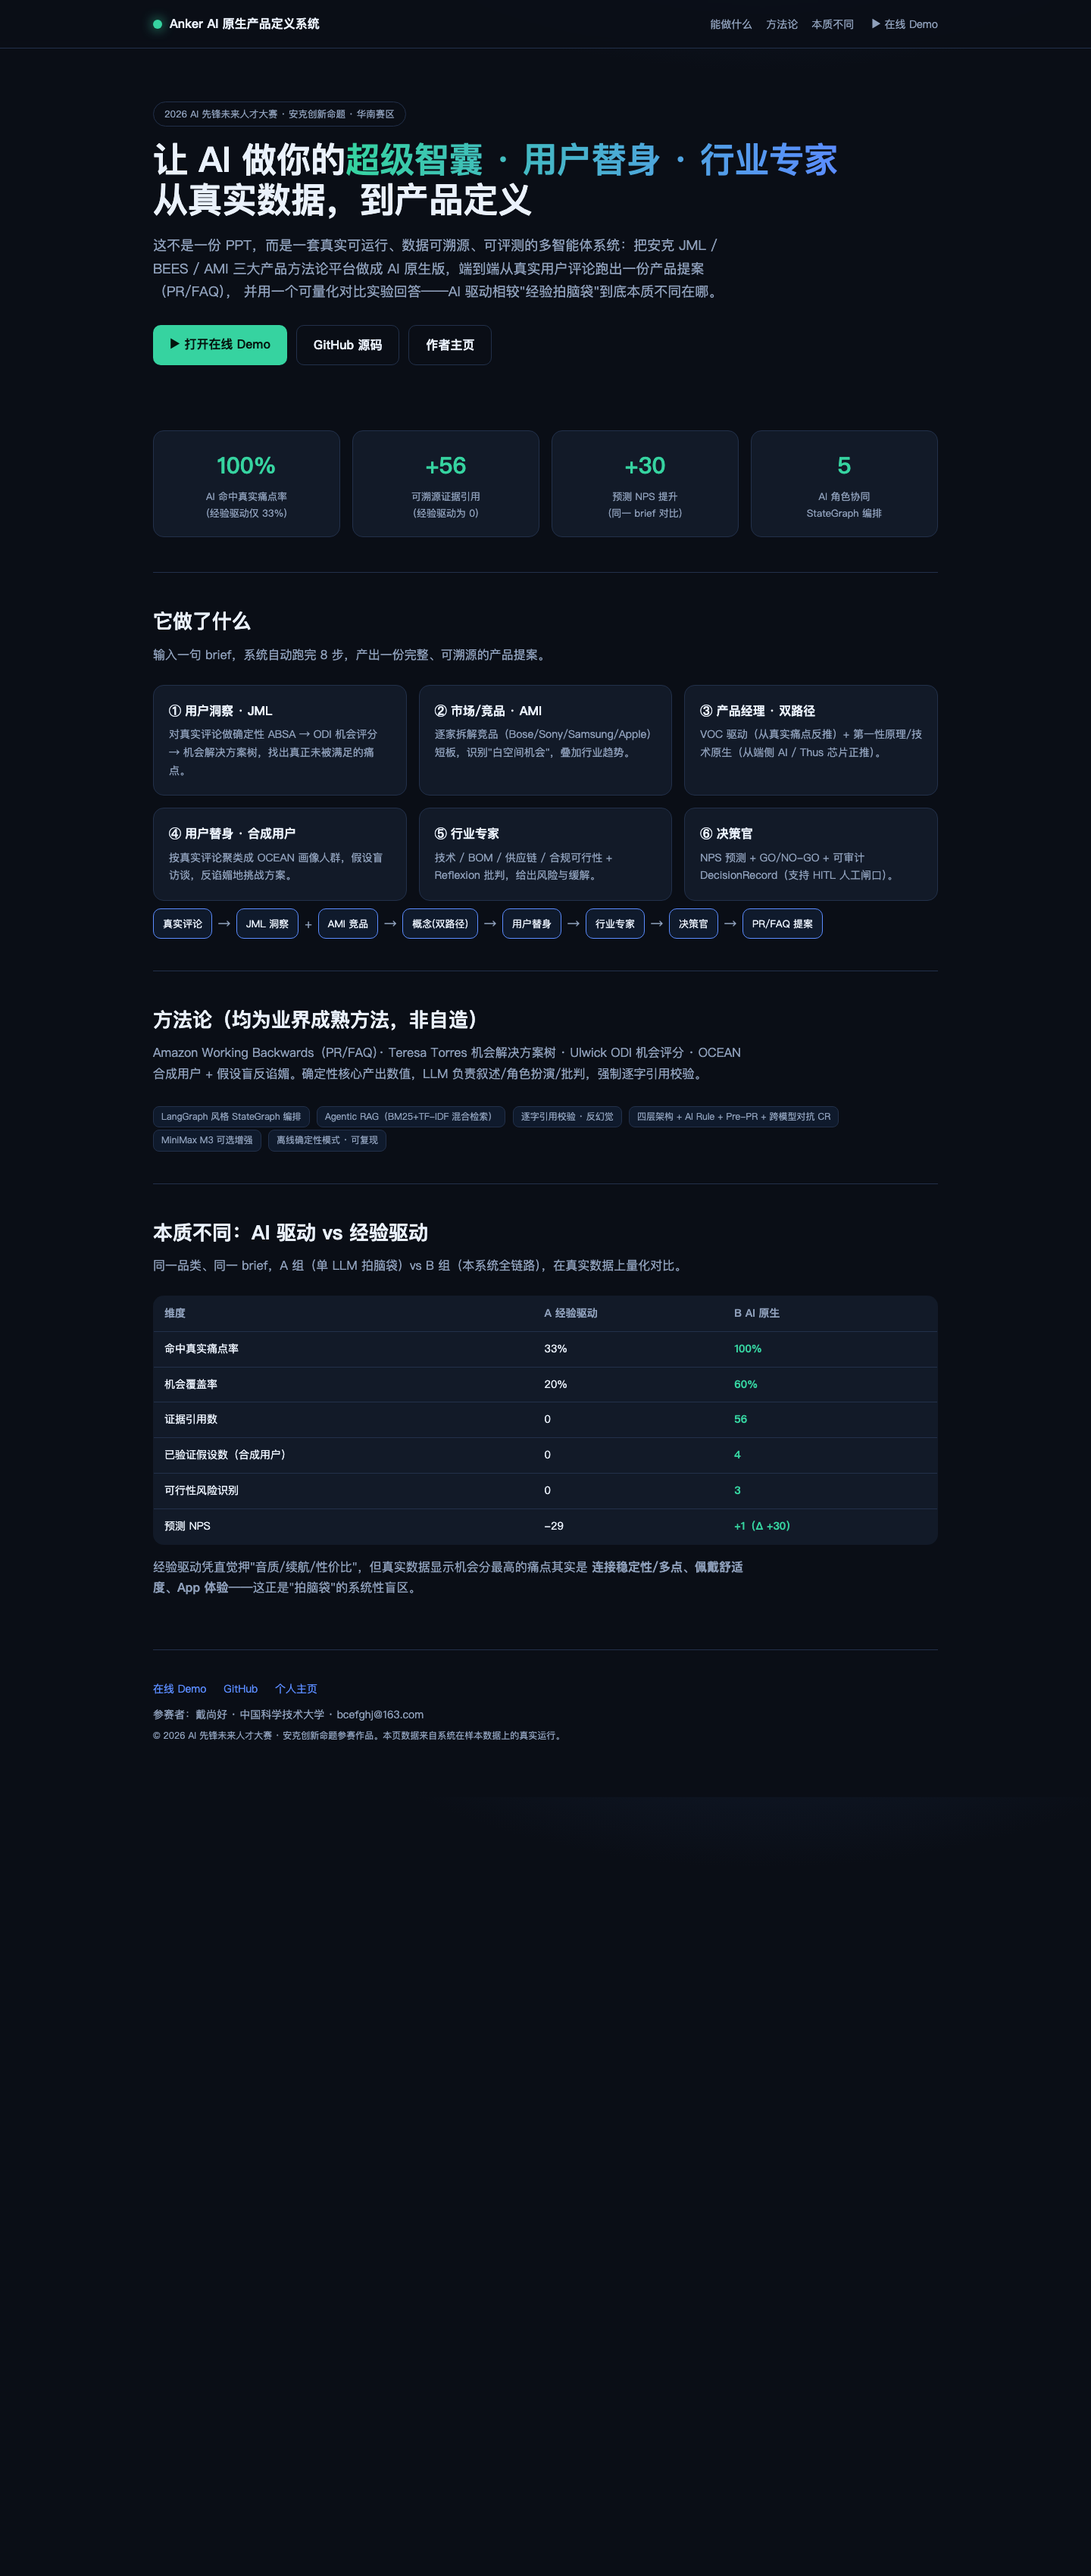
\includegraphics[width=0.86\linewidth]{../figures/landing.png}
\captionof{figure}{项目宣传页（\url{http://47.119.112.225/anker/}）}
\end{center}

\begin{center}
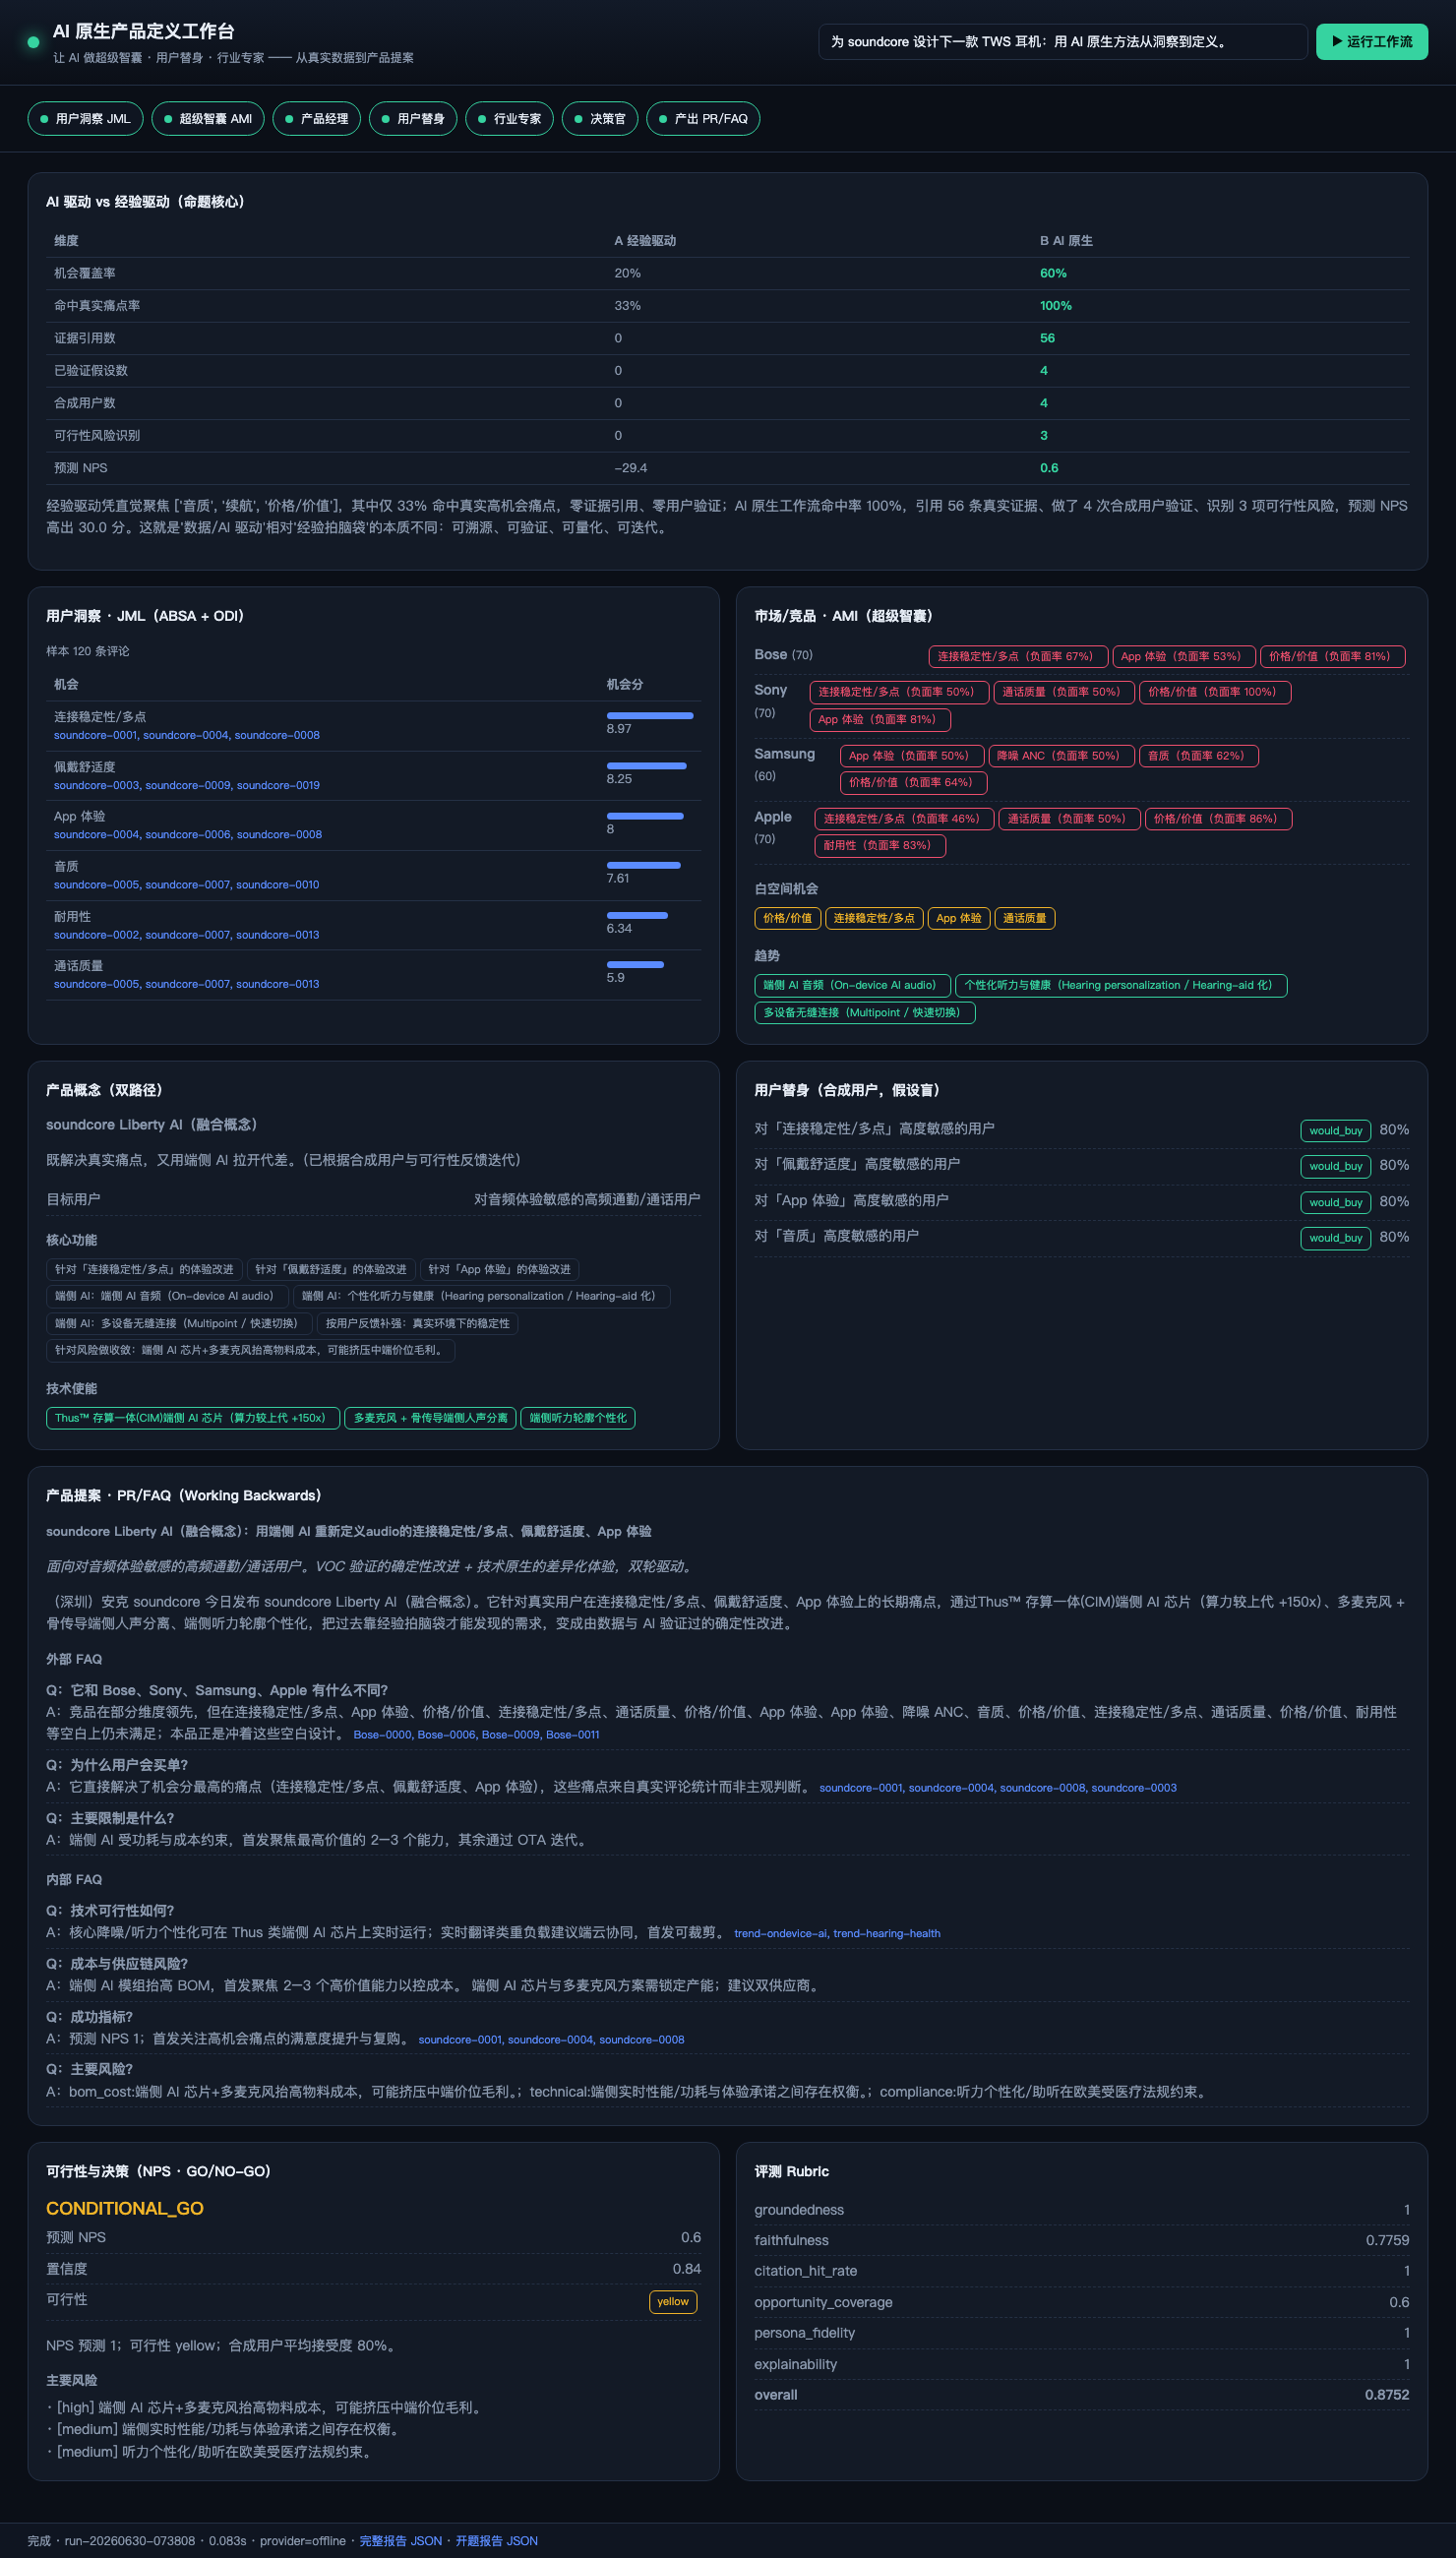
\includegraphics[width=\linewidth]{../figures/deployed_demo.png}
\captionof{figure}{线上 Demo 实跑结果（\url{http://47.119.112.225/anker/app/}）}
\end{center}

\section{链接汇总}
\begin{itemize}
\item 在线 Demo：\url{http://47.119.112.225/anker/app/}
\item 项目宣传页：\url{http://47.119.112.225/anker/}
\item 项目导航 Hub：\url{http://47.119.112.225/}
\item GitHub 源码：\url{https://github.com/bcefghj/anker-ai-product-studio}
\item 个人主页：\url{https://bcefghj.github.io}
\end{itemize}

\section{复现指南}
\begin{lstlisting}[language=bash,numbers=none]
# 1) 离线确定性模式（零网络、可复现）
pip install -r requirements.txt
python3 data/make_sample.py
PYTHONPATH=backend python3 -m anker_studio.starter.cli run
# 2) 可视化工作台
PYTHONPATH=backend python3 -m uvicorn anker_studio.starter.api:app --port 8000
# 3) 接入 MiniMax M3：在 .env 设 MINIMAX_API_KEY 并 ANKER_LLM_PROVIDER=minimax
# 4) 用真实 Amazon 评论：python3 -m anker_studio.infrastructure.data.amazon_reviews
\end{lstlisting}

\section{局限与未来工作}
\begin{itemize}
\item 合成用户与离线评分是"发现 + 排序"工具，不替代真实用户终验（与 NN/g 结论一致）；建议作为 AI 原生方法前置问题空间、把研究预算花在刀刃上。
\item 线上 Demo 默认 offline 确定性模式以保证稳定与零成本；接入 MiniMax M3 可增强叙述质量与多模态。
\item 可对接安克 AIME 平台，把本 SOP 沉淀为内部新 Agent 能力；并扩展到充电、eufy 等品类（仅需更换数据配置与 aspect 词典）。
\item 可引入更强的 ABSA 模型（BERT 类）与真实 A/B 实验闭环，进一步提升机会识别与 NPS 预测精度。
\end{itemize}

\section{结语}
本作品用一套真实可运行、可溯源、可评测的系统回答了命题：AI 原生的产品定义，不是"让 AI 帮你更快拍脑袋"，而是把产品判断
从个人经验升级为可复制的系统能力——这正是安克"用 AI 重新定义怎么想出一个好产品"的方向。
